\subsection{Vorbereitung}
Bevor der eigentliche Versuch beginnt, werden für drei periodische Funktionen
die jeweiligen Fourier-Koeffizienten berechnet. Bei den Funktionen handelt es
sich um Rechteckspannung, Sägezahnspannung und Dreieckspannung. Zur Vereinfachung
werden diese so parametrisiert, dass sie entweder gerade oder ungerade sind.
Diese Vereinfachung führt dazu, dass bei geraden Funktionen $b_\su{n}=0$ und bei
ungeraden Funktionen $a_\su{n}=0$ gür alle $n$ gilt.
\subsection{Fourier-Analyse}
Für die Fourier-Analyse von periodischen Schwingungen wird eine Schaltung wie in
Abbildung \ref{fig:ana} verwendet.
\begin{figure}[h]
  \centering
  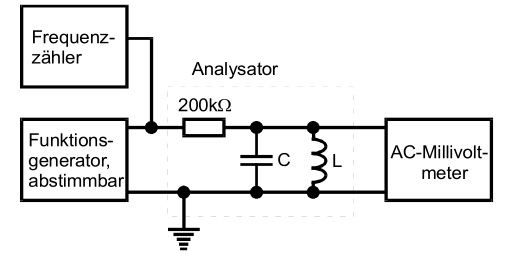
\includegraphics[width=0.8\textwidth]{bilder/analyse.jpg}
  \caption{Schaltung zur Fourier-Analyse\cite{351}}
  \label{fig:ana}
\end{figure}
Als Signalquelle dient hier ein durchstimmbarer Funktionsgenerator. Die
Transformation wird direkt vom Oszilloskop durchgeführt.

Damit genügend Peaks des Linienspektrums sichtbar werden, müssen ausreichend
Perioden angezeigt werden. Die angezeigten Peaks werden nun mit einer
Sinusspannung kalibriert und die Frequenz und die Amplitude werden notiert.
Nebenmaxima die sich bilden können, werden nicht beachtet. Die Messung wird für
alle genannten Funktionen durchgeführt.
\subsection{Fourier-Synthese}
